\begin{figure}[h]
    \centering
    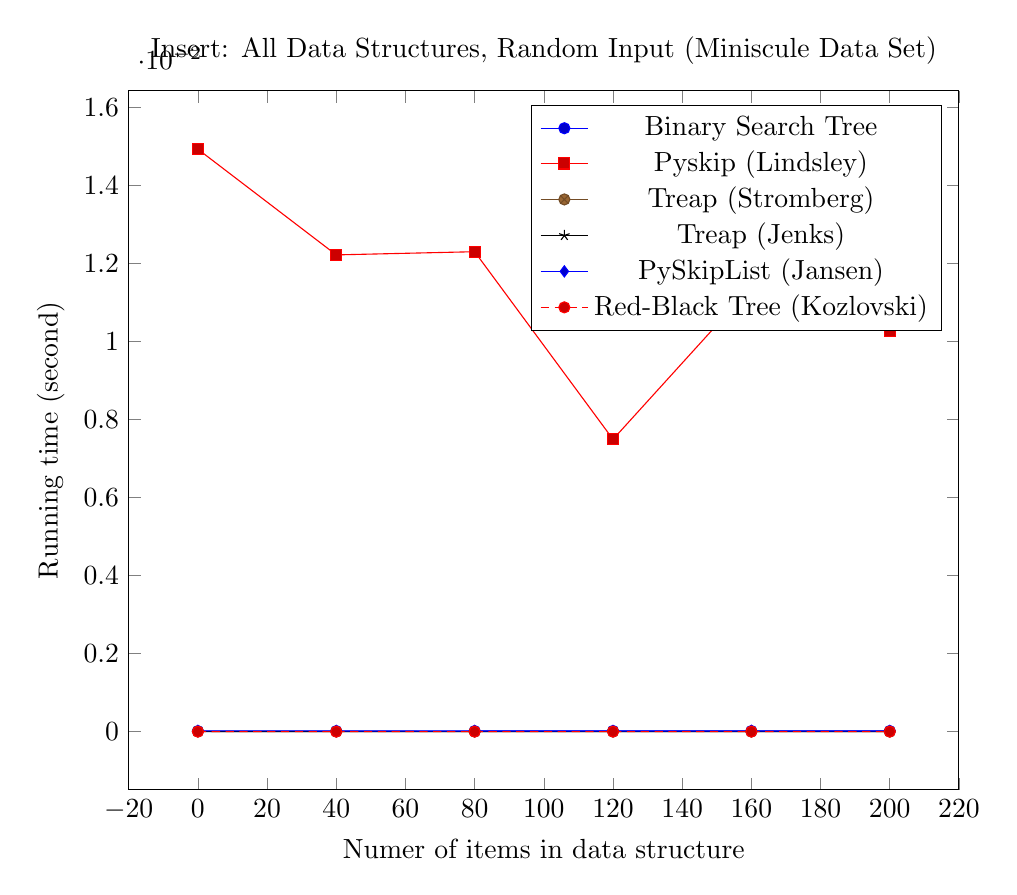
\begin{tikzpicture}
        \begin{axis}[
            xlabel={Numer of items in data structure},
            ylabel={Running time (second)},
            title={Insert: All Data Structures, Random Input (Miniscule Data Set)},
            width=\textwidth
        ]
		\addplot coordinates {
			(0, 1.7377816930697067e-05)
			(40, 1.7528404599076453e-05)
			(80, 1.7528404599076453e-05)
			(120, 1.9696867023633047e-05)
			(160, 1.8853576080779533e-05)
			(200, 1.8913811148024705e-05)
		};
		\addplot coordinates {
			(0, 0.014933658602696909)
			(40, 0.012224164803144432)
			(80, 0.012305723084336685)
			(120, 0.007496284249282859)
			(160, 0.011405178709915375)
			(200, 0.010274807436019096)
		};
		\addplot coordinates {
			(0, 7.679971087171112e-06)
			(40, 5.36092099423513e-06)
			(80, 4.276689781868015e-06)
			(120, 4.3670423830022285e-06)
			(160, 5.180215792144338e-06)
			(200, 5.270568393100916e-06)
		};
		\addplot coordinates {
			(0, 2.680460497117565e-06)
			(40, 2.4395202277815995e-06)
			(80, 2.2286974919794033e-06)
			(120, 2.349167626647386e-06)
			(160, 2.108227357133785e-06)
			(200, 2.590107896160987e-06)
		};
		\addplot coordinates {
			(0, 2.1112391106292704e-05)
			(40, 2.0118512494882167e-05)
			(80, 1.930533908574006e-05)
			(120, 1.9516161821542254e-05)
			(160, 2.0238982629727788e-05)
			(200, 1.9365574153162868e-05)
		};
		\addplot coordinates {
			(0, 2.7406955645403743e-06)
			(40, 3.0418709011215126e-06)
			(80, 3.1623410359671313e-06)
			(120, 3.4936339062596743e-06)
			(160, 3.523751439971079e-06)
			(200, 3.5237514401487145e-06)
		};
        \legend{Binary Search Tree, Pyskip (Lindsley), Treap (Stromberg), Treap (Jenks), PySkipList (Jansen), Red-Black Tree (Kozlovski)}
        \end{axis}
    \end{tikzpicture}
    \caption{Average of 10 operations, benchmarked every 40, starting at 0.}
\end{figure}